%!TEX root = ../../thesis.tex

\section{Interaction frame hypothesis}
\label{chapter:limitations:framehypothesis}

\question{How to leverage from the pre-defined unique interaction frame?}

Until now we have assumed that the interaction frame, which specifies the details of the interaction between the human and the machine was known. In this frame only the meaning of the signal was unknown. We now open this side of the interaction and considered the case where multiple interaction are define, but only one of them account for the interaction between the human and the machine.

We will use a very simple example to illustrate the problem and show computational results on the same simple scenario. We consider that the agent lives in the line word as defined in chapter~\ref{chapter:lfui::symmetries}, where the agent has access to the ``no move'' action in order to remove the symmetry problem. The agent knowns it should reach either of the two edges of the world, G1 or G2. And the agent knowns that the teacher is providing either feedback or guidance instructions. To handle this new hidden information we will rely again on our interpretation hypothesis process. This time, one hypothesis will be the combination of one task hypothesis and one frame hypothesis.  For our simple example, it results in having four hypothesis.

The result of the labeling process is shown in Figure~\ref{fig:multipleframeexplainedfeedback} for a teacher providing feedback instruction according the task G1 (of course the agent do not have access to this information). The hypothesis that labels the signals according to the task G1 and the feedback frame is the one whose signal-labels pair match better with he underlying structure of the data. Indeed for the guidance case, the labeling process for hypothesis G1 is always giving a ``left'' label whether or not the agent is moving away or closer to the target which allow to differentiate between feedback and guidance case. To differentiate between G1 and G2, the same principle than the one described in chapter~\ref{chapter:lfui::symmetries} applies.

\begin{figure}[!ht]
\centering
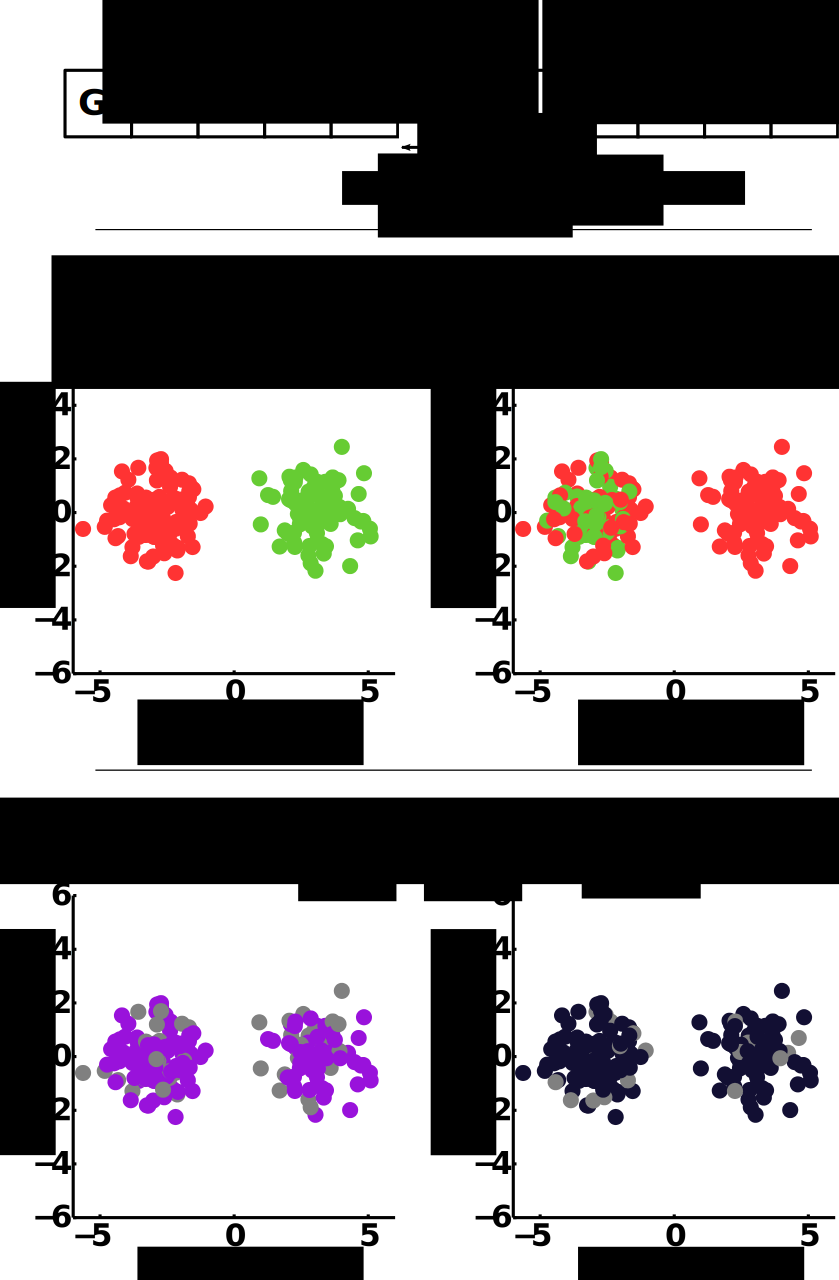
\includegraphics[width=\twoplanningwidth\columnwidth]{\visualspdf/multiple_frame/multiple_frame_feedback.pdf}
\caption{Illustration of the labelling porcess on both task and interaction frame hypothesis. The agent can perform right, left, or a ``no move'' action. The agent receive feedback on its action in the line word according to G1 . The agent do not known which task (G1 or G2) neither which interaction scheme the teacher is following (feedback or guidance). The result of the labeling process allow to identify the hypothesis on task G1 and feedback frame as the more likely.}
\label{fig:multipleframeexplainedfeedback}
\end{figure} 

Considering now that the teacher is providing guidance instruction according the task G1, the results of the labeling process can be seen in Figure~\ref{fig:multipleframeexplainedguidance}. The same explanation than for Figure~\ref{fig:multipleframeexplainedfeedback} applies. 

\begin{figure}[!ht]
\centering
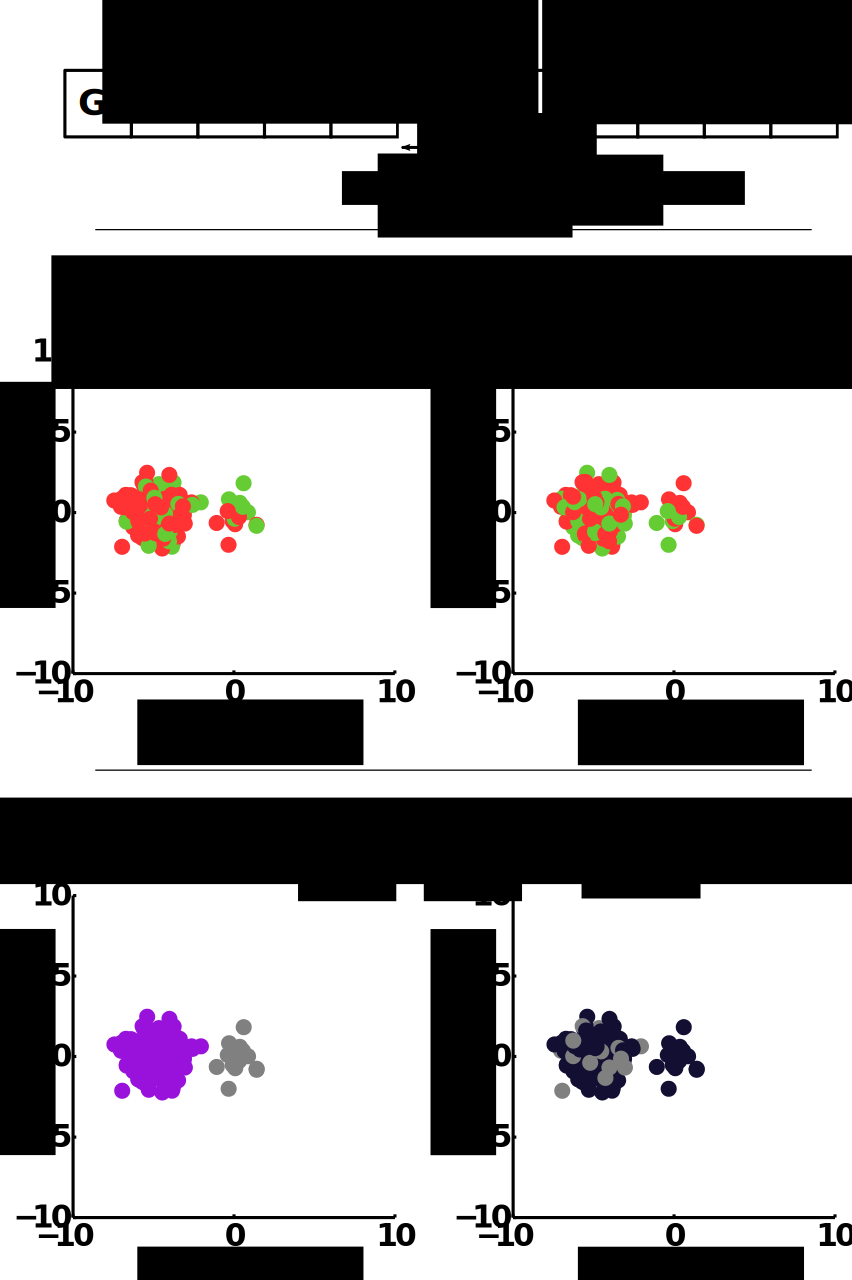
\includegraphics[width=\twoplanningwidth\columnwidth]{\visualspdf/multiple_frame/multiple_frame_guidance.pdf}
\caption{Illustration of the labelling porcess on both task and interaction frame hypothesis. The agent can perform right, left, or a ``no move'' action. The agent receive guidance instruction on its action in the line word according to G1 . The agent do not known which task (G1 or G2) neither which interaction scheme the teacher is following (feedback or guidance). The result of the labeling process allow to identify the hypothesis on task G1 and guidance frame as the more likely.}
\label{fig:multipleframeexplainedguidance}
\end{figure} 

We now verify that the algorithm works in practice. We consider the same line world scenario as described above. For our experiments, the simulated teacher select randomly a target (G1 or G2) and an interaction frame (feedback or guidance). The agent is using our uncertainty based planning method as well as the same setting as described in chapter~\ref{chapter:planning:method}. We ran 100 simulations


Figure~\ref{fig:multipleframeall} shows the evolution of our probability measure of the correct combination of task and interaction frame, which is adapted from Equation~\ref{eq:probapairwise} in chapter~\ref{chapter:lfui:confidence} (minimum of pairwise normalized likelihood) where each hypothesis is a combination of task and interaction frame. After 200 steps, all our experiments identified with probability 1 the correct combination of task and interaction frame. In practice, in our previous experiments, we used a confidence threshold of 0.9, under this condition most of our experiments would have identified the task in slighlty more than 50 steps.

\begin{figure}[!ht]
\centering
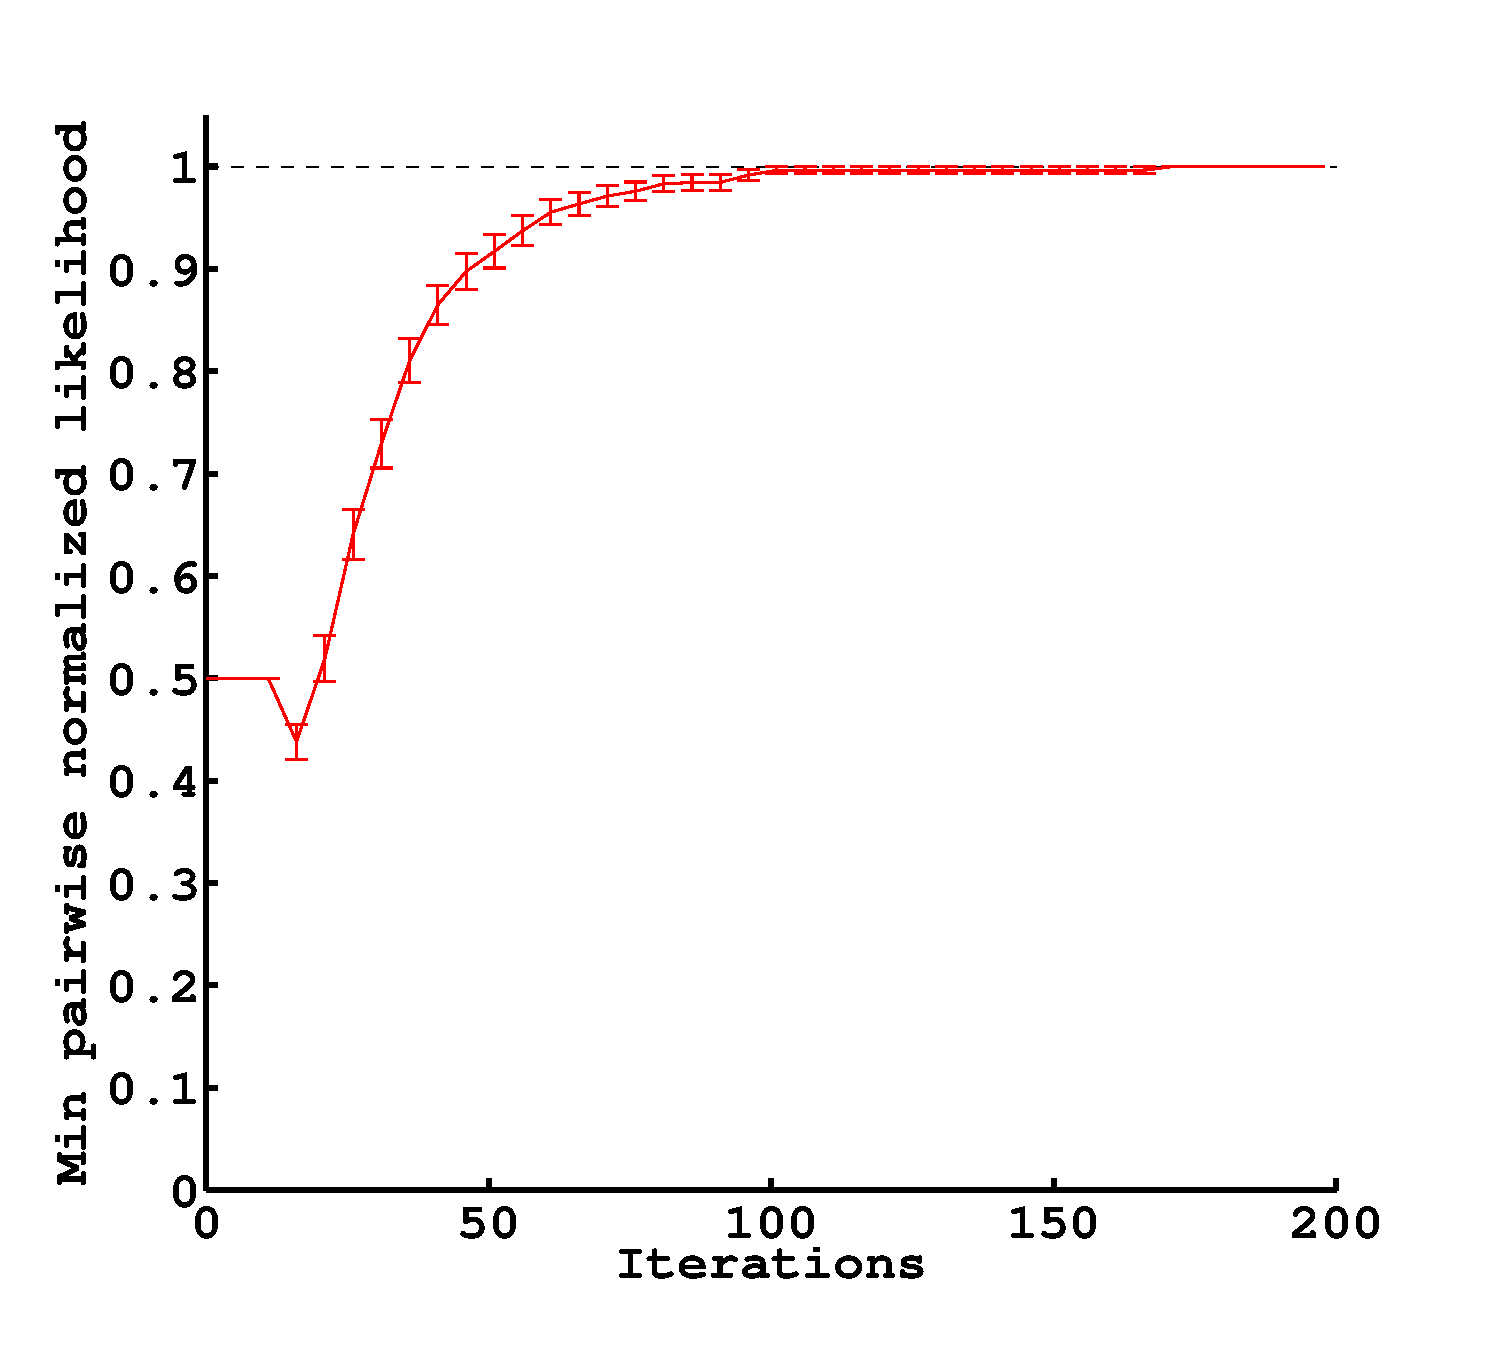
\includegraphics[width=\plotsize\columnwidth]{\imgpath/multiple_frame/multiple_frame_all_teacher.eps}
\caption{Evolution of the minimum of pairwise normalized likelihood for the correct hypothesis. After 200 steps, all our experiments identified with probability 1 the correct combination of task and interaction frame. Most of the experiments would have identified the task slighlty more than 50 steps with a confidence threshold of 0.9.}
\label{fig:multipleframeall}
\end{figure} 

We analyses in Figure~\ref{fig:multipleframefeedbackvsguidance} independently the case where the teacher was using the feedback (left) and guidance frame (right). We note that the behavior are the same for bot condition. only the guidance case took a bit longer for all hypothesis to converge to the correct task.

\begin{figure}[!ht]
\centering
\includegraphics[width=0.49\columnwidth]{\imgpath/multiple_frame/multiple_frame_feedback_teacher.eps}
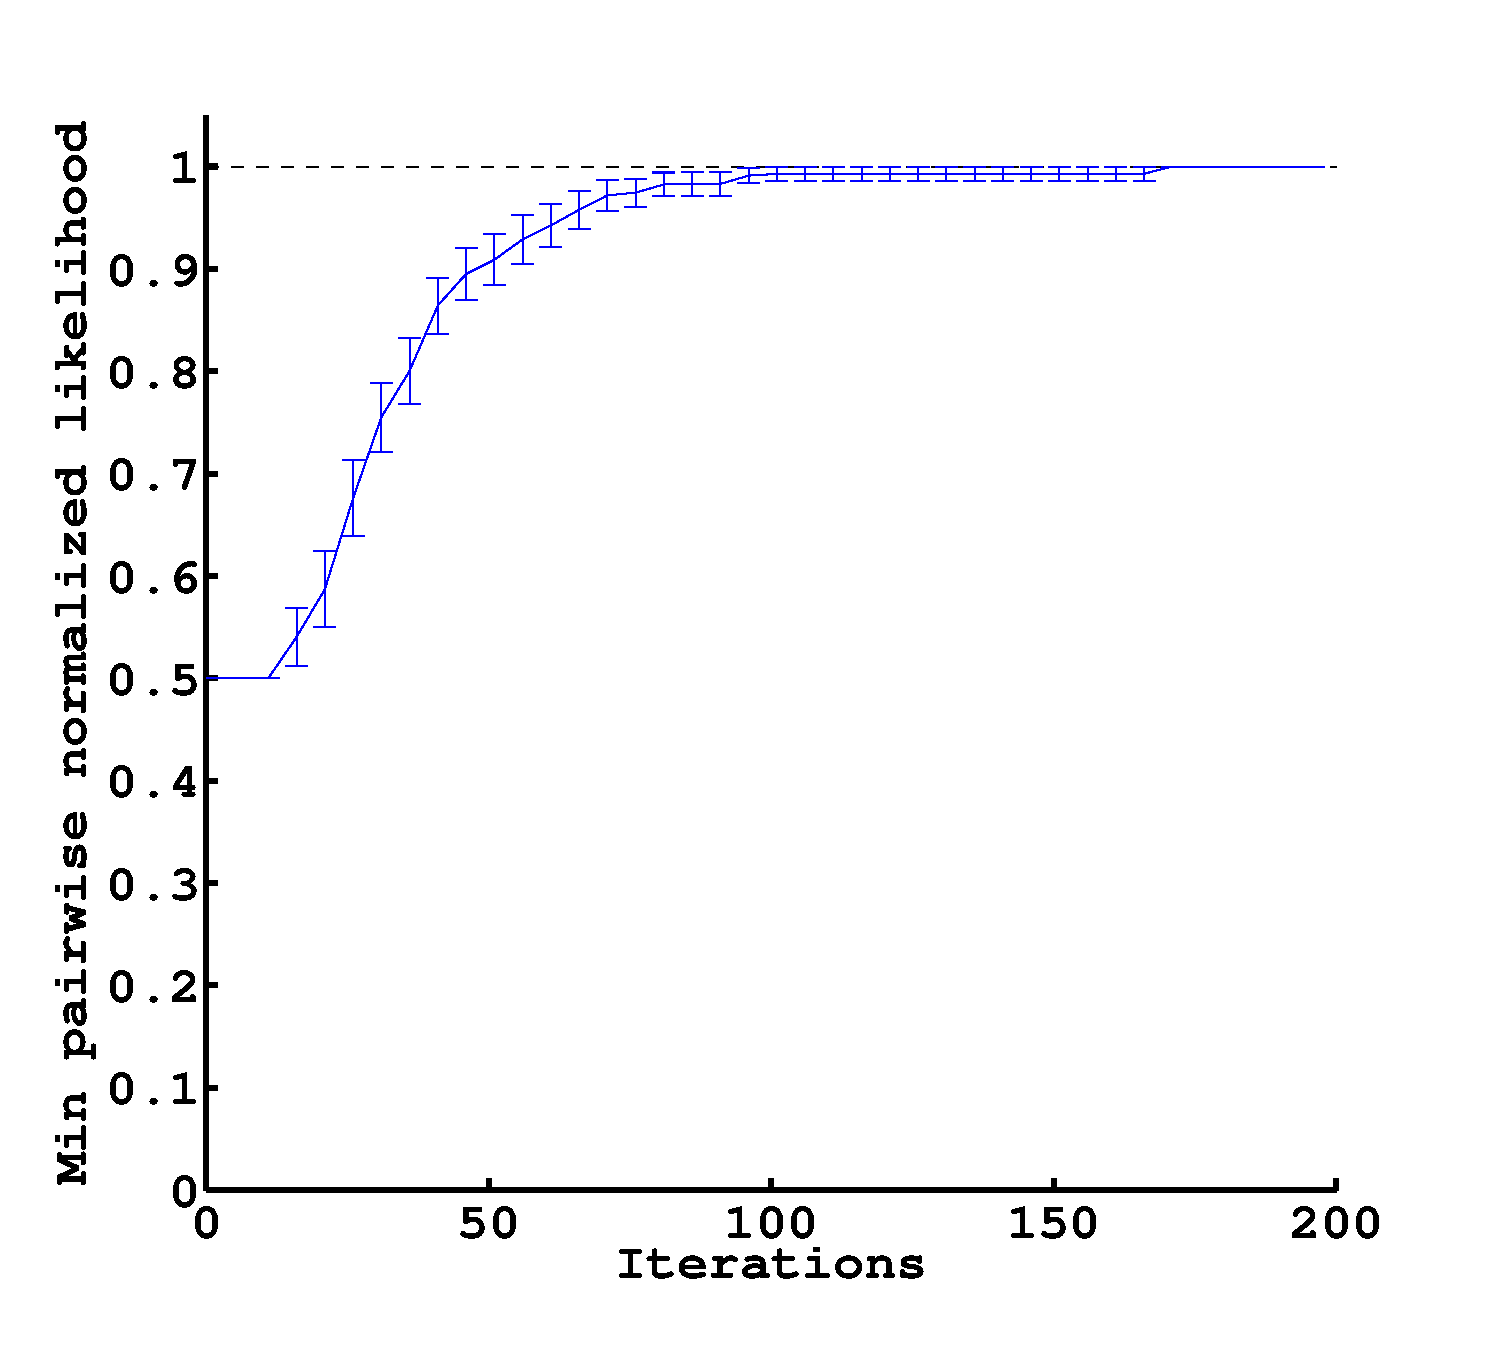
\includegraphics[width=0.49\columnwidth]{\imgpath/multiple_frame/multiple_frame_guidance_teacher.eps}
\caption{Evolution of the minimum of pairwise normalized likelihood for the correct hypothesis if the teacher provided feedback (left) or guidance (right) instruction. After 200 steps, all our experiments identified with probability 1 the correct combination of task and interaction frame. Most of the experiments would have identified the task in slighlty more than 50 steps with a confidence threshold of 0.9.}
\label{fig:multipleframefeedbackvsguidance}
\end{figure} 


From those results in a simplistic environment, we can envision that following our interpretation hypothesis method for both task and interaction frame combination, one could start learning a task from unlabeled instructions and undefined interaction frames. In the end, our system would not only learn the task and the signal to meaning mapping, but also the interaction protocol used by the teacher.

Considering our example in section~\ref{chapter:limitation:continoustask}, an other potential use of the frame hypothesis scheme describe above would be to consider two different referential for the cardinal signal direction. Considering for example two cases, either the guidance signals are relative to the true North magnetic pole, either they are related to the current position of the user relative to the agent, or even relative to the current orientation of the robot (where going North would mean go straight). This experiment performed with a real robot, real users, considering a tablet, and different interaction frames has great potential to demonstrate the potential application of our work to a broader audience.

Finally a particle filter based method as used in section~\ref{chapter:limitations:continoushypothesis} for dealing with continuous task could be considered for dealing with a continuous set of interaction frame. For example, in our example of section~\ref{chapter:limitations:continousstate}, we used a parameterized frame that combines feedback and guidance frame (see Equation~\ref{eq:mixedfeedbackguidance}). By generating, testing, and resampling a set of those interaction frames we may be able to learn, not only the task and the signal to meaning mapping, but also the details of the interaction protocol used by the teacher. For example, in the experiment of section~\ref{chapter:limitations:continousstate} we may identify automatically the $\beta$ parameter of Equation~\ref{eq:mixedfeedbackguidance}.